\documentclass{article}

\usepackage{fullpage}
\usepackage{url}
\usepackage{bbm}
\usepackage{graphicx}
\usepackage{amsmath}
\usepackage{physics}
\usepackage{mathtools}
\usepackage{bbold}
\usepackage{slashed}
\usepackage{pxfonts}
\usepackage{multicol}
\usepackage{mathptmx}
\usepackage{simplewick}
\usepackage{placeins}

\usepackage{lmodern}
\usepackage[T1]{fontenc}
\usepackage[fontsize=13.5pt]{fontsize}

\DeclareMathOperator{\erfi}{erfi}
\newcommand{\R}{\ensuremath{\mathbb{R}}}
\newcommand{\C}{\ensuremath{\mathbb{C}}}

\title{Quantum Field Theory I Excercise 2}
\author{Idan Stark}
\date{\today}

\begin{document}
\maketitle

\section{Perturbation theory for Gaussian integrals}
\subsection{The $x^4$ interaction up to second order in $\lambda$}
Let us look at the potential
\begin{equation}
    V(x) = \frac{1}{4!}\sum_{i=1}^n x_i^4
\end{equation}
In zeroth order:
\begin{equation}
    \langle V^0(x) \rangle = \langle 1 \rangle = Z(0)
\end{equation}
In first order:
\begin{equation}
    \langle V(x) \rangle = \frac{1}{4!} \sum_{i=1}^n \langle x_i^4 \rangle
\end{equation}
Using Wick's theorem and from the symmetry of the $x_i^4$, we can see that there are $3$ potential pairings, and for all of them we get $\Delta_{ii}^2$:
\begin{equation}
    \langle V(x) \rangle = \frac{1}{8} \sum_{i=1}^n \Delta_{ii}^2
\end{equation}
Similarly, in second order we have four cases:
\begin{itemize}
    \item If $i = j$, there are $7\cdot5\cdot3 = 105$ options for pairings.
    \item If $i \ne j$, there are three options:
    \begin{itemize}
        \item Each $x_i$ is paired with one $x_j$, resulting in four $x_ix_j$ pairs. There are $4!$ permutations in this option (just order the $x_i$s in a row and then permutate the order of the $x_j$).
        \item There are two $x_i x_j$ pairs, and the other are connected to themselves: $x_ix_i$ and $x_jx_j$. There are six options for the internally connected pair in each index, then two options for the permutation of the two $x_ix_j$ pairs. In total $6\cdot6\cdot2 = 72$ options.
        \item Finally, we have the unconnected option where all pairs are with themselves: two $x_ix_i$ pairs and two $x_jx_j$ pairs. There are three options for the pairing in each of the indices, leading to $3\cdot3 = 9$ options.
    \end{itemize}
\end{itemize}
So, the second order contribution is:
\begin{equation}
    \langle V^2(x) \rangle = \frac{1}{4!^2} \sum_{i,j=1}^n \langle x_i^4x_j^4 \rangle = \frac{105}{4!^2}\sum_{i=1}^n \Delta_{ii}^4 + \frac{1}{4!^2}\sum_{i,j=1, i\ne j}^n (9 \Delta_{ii}^2 \Delta_{jj}^2 + 72\Delta_{ii}\Delta_{jj}\Delta_{ij}^2 + 4! \Delta_{ij}^4)
\end{equation}
In total, we get:
\begin{equation}
\begin{gathered}
    \frac{Z(\lambda)}{Z(0)} = 1 - \frac{1}{8} \left[\sum_{i=1}^n \Delta_{ii}^2\right] \lambda + \\ + \frac{1}{2}\left[\frac{35}{192}\sum_{i=1}^n \Delta_{ii}^4 + \sum_{i,j=1, i\ne j}^n \left(\frac{1}{64} \Delta_{ii}^2 \Delta_{jj}^2 + \frac{1}{8}\Delta_{ii}\Delta_{jj}\Delta_{ij}^2 + \frac{1}{24}\Delta_{ij}^4\right)\right]\lambda^2 + O(\lambda^3) = \\ =
    1 - \frac{1}{8} \left[\sum_{i=1}^n \Delta_{ii}^2\right] \lambda + \\ + \left[\frac{35}{384}\sum_{i=1}^n \Delta_{ii}^4 + \sum_{i,j=1, i\ne j}^n \left(\frac{1}{128} \Delta_{ii}^2 \Delta_{jj}^2 + \frac{1}{16}\Delta_{ii}\Delta_{jj}\Delta_{ij}^2 + \frac{1}{48}\Delta_{ij}^4\right)\right]\lambda^2 + O(\lambda^3) 
\end{gathered}
\end{equation}
\newpage
\subsection{Feynman diagrams}
\begin{figure}[!htbp]
    \centering
    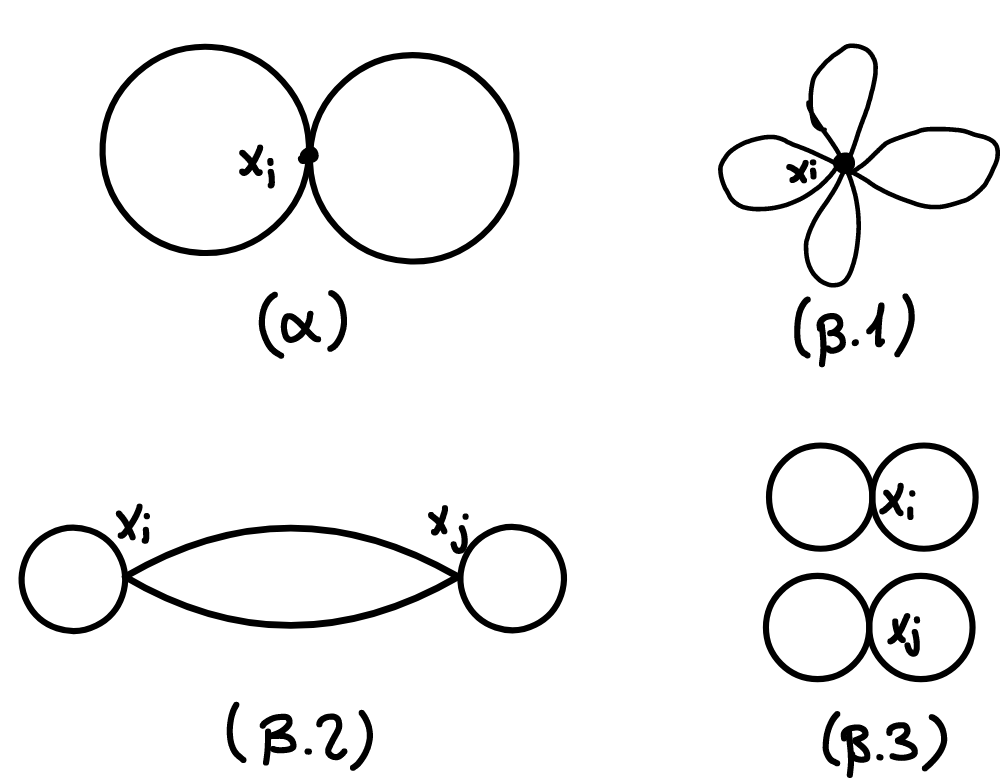
\includegraphics[width=0.5\textwidth]{figures/ex1.png}
    \caption{These are the first and second order contributions to the correlation function. Diagram $(\alpha)$ shows the first order contribution, with one vertex and two loops. Diagrams $(\beta.1)$, $(\beta.2)$ and $(\beta.3)$ show the second order contributions, with two vertices and four loops, two loops and two internal lines, and four internal lines respectively.}
\end{figure}
\subsection{$W(\lambda)$}
Let us now compute the $\ln$ of the correlation function:
\begin{equation}
\begin{gathered}
    W(\lambda) = \ln\Bigg(1 - \frac{1}{192} \left[\sum_{i=1}^n \Delta_{ii}^2\right] \lambda + \\ + \left[\frac{35}{384}\sum_{i=1}^n \Delta_{ii}^4 + \sum_{i,j=1, i\ne j}^n \left(\frac{1}{128} \Delta_{ii}^2 \Delta_{jj}^2 + \frac{1}{16}\Delta_{ii}\Delta_{jj}\Delta_{ij}^2 + \frac{1}{48}\Delta_{ij}^4\right)\right]\lambda^2 + O(\lambda^3) \Bigg)
\end{gathered}
\end{equation}
We can expand using $\ln(1 - x) \approx - x - \frac{1}{2}x^2$, but keeping only up to second term in $\lambda$:
\begin{equation}
\begin{gathered}
    W(\lambda) \approx - \frac{1}{8} \left[\sum_{i=1}^n \Delta_{ii}^2\right] \lambda + \left[\frac{35}{384}\sum_{i=1}^n \Delta_{ii}^4 + \sum_{i,j=1, i\ne j}^n \left(\frac{1}{128} \Delta_{ii}^2 \Delta_{jj}^2 + \frac{1}{16}\Delta_{ii}\Delta_{jj}\Delta_{ij}^2 + \frac{1}{48}\Delta_{ij}^4\right)\right]\lambda^2 - \\ -
    \frac{1}{2}\left(\frac{1}{8}\left[\sum_{i=1}^n \Delta_{ii}^2\right] \lambda\right)^2 = \\ =
    - \frac{1}{8} \left[\sum_{i=1}^n \Delta_{ii}^2\right] \lambda + \left[\frac{1}{12}\sum_{i=1}^n \Delta_{ii}^4 + \sum_{i,j=1, i\ne j}^n \left(\frac{1}{16}\Delta_{ii}\Delta_{jj}\Delta_{ij}^2 + \frac{1}{48}\Delta_{ij}^4\right)\right]\lambda^2
\end{gathered}
\end{equation}
As we can see, the disconnected term $\Delta_{ii}^2\Delta_{jj}^2$ vanished, and the single vertex term $\Delta_{ii}^4$ changed its prefactor.

\newpage
\section{Potential between two static sources}
In this section we look at a source in the free scalar theory:
\begin{equation}
    \mathcal{L} = \frac{1}{2}\left(\partial_\mu \phi\right)^2 - \frac{1}{2}m^2\phi^2
\end{equation}
where the source represents two particles at a fixed distance $R$:
\begin{equation}
    J(t, \vec{x}) = \Theta(T - t)\theta(t)\left[
        q_1\delta^3(\vec{x}) + q_2\delta^3(\vec{x} - \vec{R})
    \right]
\end{equation}
We found in class that
\begin{equation}
    Z[J] = Z[0]\exp[-\frac{1}{2}\int d^4x d^4y J(x)\Delta_F(x - y)J(y)]
\end{equation}
Plugging the source into the integral in the exponent yields
\begin{equation}
\begin{gathered}
    \int d^4x d^4y J(x)\Delta_F(x - y)J(y) = \\ =
    \int d^4x d^4y \Theta(T - x^0)\theta(x^0)\left[
        q_1\delta^3(\vec{x}) + q_2\delta^3(\vec{x} - \vec{R})
    \right] \times \\ \times
    \Delta_F(x - y)
    \Theta(T - y^0)\theta( y^0)\left[
        q_1\delta^3(\vec{y}) + q_2\delta^3(\vec{y} - \vec{R})
    \right]
\end{gathered}
\end{equation}
This spatial integrals give two options up to a coordinate transformation: $\vec{x} = \vec{y}$ or $\vec{x} - \vec{y} = -\vec{R}$:
\begin{equation}
    = \int_0^T dx^0 \int_0^T dy^0 \left[
        \left(q_1^2 + q_2^2\right)\Delta_F(x^0 - y^0, \vec{0}) +
        2q_1q_2\Delta_F(x_0 - y_0, -\vec{R})
    \right]
\end{equation}
The first term is a constant (independent of $R$), while the second part integrates to
\begin{equation}
\begin{gathered}
    \int_0^T dx^0 \int_0^T dy^0 \Delta_F(x_0 - y_0, -\vec{R}) = \int_0^T dx^0 \int_0^T dy^0 \int \frac{d^4k}{(2\pi)^4} \frac{ie^{-i(k^0(x^0 - y^0) - \vec{k}\cdot\vec{R})}}{k^2 - m^2 + i\epsilon} = \\ =
    \int \frac{dk^0}{2\pi} \int_0^T dx^0 \int_0^T dy^0 e^{-ik^0(x^0 - y^0)} \int \frac{d^3k}{(2\pi)^3} \frac{ie^{i\vec{k}\cdot\vec{R}}}{k^2 - m^2 + i\epsilon}
\end{gathered}
\end{equation}
Starting from the time integrals:
\begin{equation}
\begin{gathered}
    \int_0^T dx^0 \int_0^T dy^0 e^{-ik^0(x^0 - y^0)} = \\ =
    -\frac{1}{ik^0} \int_0^T dx^0 e^{-ik^0(x^0 - T)} - e^{-ik^0(x^0 - 0)} = \\ =
    \frac{1}{(k^0)^2} \left[
        e^{-ik^0(T - T)} - e^{-ik^0(T - 0)} -
        e^{-ik^0(0 - T)} + e^{-ik^0(0 - 0)}
    \right] = \\ =
    \frac{2}{(k^0)^2} \left[1 - \cos(k^0 T)\right] = \frac{4\sin^2\left(\frac{k^0T}{2}\right)}{(k^0)^2}
\end{gathered}
\end{equation}
But, since for every $f(x)$:
\begin{equation}
    \lim_{a \rightarrow \infty}\int dx \frac{\sin^2(ax)}{(ax)^2}f(x) = 
    \lim_{a \rightarrow \infty} a ^{-1}\int d\xi \frac{\sin^2(\xi)}{\xi^2}f\left(\frac{\xi}{a}\right) = a^{-1} \pi f(0)
\end{equation}
We can write:
\begin{equation}
    \lim_{a \rightarrow \infty}\frac{\sin^2(ax)}{(ax)^2} = a^{-1}\pi \delta(x)
\end{equation}
Which means that for large enough $T$:
\begin{equation}
    \frac{4\sin^2\left(\frac{k^0T}{2}\right)}{(k^0)^2} =
    T^2\frac{\sin^2\left(\frac{k^0T}{2}\right)}{(T k^0/2)^2} \rightarrow 2\pi T \delta(k^0)
\end{equation}
Pluggin this now into the $k^0$ integral yields:
\begin{equation}
\begin{gathered}
    \int \frac{dk^0}{2\pi} \int_0^T dx^0 \int_0^T dy^0 e^{ik^0(x^0 - y^0)} \int \frac{d^3k}{(2\pi)^3} \frac{ie^{i\vec{k}\cdot\vec{R}}}{k^2 - m^2 + i\epsilon} = \\ =
    -T \int \frac{d^3k}{(2\pi)^3} \frac{ie^{i\vec{k}\cdot\vec{R}}}{\vec{k}^2 + m^2 + i\epsilon} = \\ =
    -T \int \frac{k^2 dk d(\cos(\theta)) d\varphi}{(2\pi)^3} \frac{ie^{ikR\cos(\theta)}}{k^2 + m^2} = \\ =
    -iT \int \frac{k^2 dk d(\cos(\theta))}{(2\pi)^2} \frac{e^{ikR\cos(\theta)}}{k^2 + m^2} = \\ =
    -\frac{T}{R} \int_0^\infty \frac{k dk}{(2\pi)^2} \frac{e^{ikR} - e^{-ikR}}{k^2 + m^2} = \\ = -\frac{T}{R}\frac{i\pi}{(2\pi)^2}e^{-mR} = -\frac{iT e^{-mR}}{4\pi R}
\end{gathered}
\end{equation}
Where in the last step we used the reverse Fourier transform of $k / (k^2 + m^2)$. This result gives:
\begin{equation}
    Z[J] = Z[0]\exp[\frac{1}{2}\cdot 2 q_1 q_2 \frac{iT}{4\pi R}e^{-mR} + \text{const}] =
    Z[0]\exp[i q_1 q_2 T\frac{e^{-mR}}{4\pi R} + \text{const}]
\end{equation}
Defining
\begin{equation}
    V(R) = -q_1q_2\frac{e^{-mR}}{4\pi R}
\end{equation}
We get:
\begin{equation}
    Z[J] = Z[0]\exp[-iTV(R) + \text{const}]
\end{equation}
\subsection{Discussion}
The above potential has the following interesting limits:
\begin{itemize}
    \item If $m = 0$, we get the Lorentz potential. So, the potential agrees with the limit of massless particles transmiting square-inverse forces.
    \item If $R \gg m^{-1}$, the potential is zero, meaning that particles that are too far apart will not interact. In fact, in that since the mass dictated the interaction distance.
    \item The additional constant is proportional to the sum of squares of the two charges. It can thought of as the interaction of each particle with itself, in the duration of the time.
\end{itemize}

\newpage
\section{The “phi-cubed” Scalar Field Theory}
In this section we look at the theory with the Lagrangian
\begin{equation}
    \mathcal{L} = \frac{1}{2}\left(\partial_\mu \phi\right)^2 - \frac{1}{2}m^2\phi^2 - \frac{\mu}{3!}\phi^3
\end{equation}
\subsection{Position space Feynman rules}
We can find the Feynman rules similary to the $\phi^4$ theory. Looking at a general correltion function
\begin{equation}
\begin{gathered}
    \langle T \phi(x_i) \cdots \phi(x_n) \rangle = \int \mathcal{D}\phi T \phi(x_i) \cdots \phi(x_n) \exp[i \int d^4x \mathcal{L}_0 - \frac{\mu}{3!}\phi^3] = \\ =
    \Delta_F(x_1 - x_2) + \left(-\frac{i\mu}{3!}\right) \int \mathcal{D}\phi \phi(x_i) \cdots \phi(x_n) \int d^4x \phi^3(x) + \cdots
\end{gathered}
\end{equation}
Since the three fields in the interaction point $x$ are interchangable, the factor $3!$ cancels out. This gives the following Feynman rules:
\begin{itemize}
    \item Propagators: each line in the diagram gives a Feynman propagator $\Delta_F(x - y)$.
    \item Vertices: each vertex gives a factor of, and an integral over an internal point $-i\mu \int d^4z$.
    \item Each external leg gives a factor of 1.
    \item Divide by symmetry factor.
\end{itemize}
\subsection{Momentum space Feynman rules}
In momentum space, each Feynman propegator is replaced by its Fourier transform, the vertices spatial integrals disapear, and external points get a momentum final state:
\begin{itemize}
    \item Propagators: each line in the diagram gets a momentum $p$ and gives the Fourier transform of the Feynman propegator $\frac{i}{p^2 - m^2 + i\epsilon}$.
    \item Each external point gives a factor $e^{-ipx}$.
    \item Vertices: each vertex gives a factor of $-i\mu$ and a $\delta$ function over the sum of momenta going into the vertex (momenta going outwards get a minus sign) for momentum conservation.
    \item Integrate over all undetermined momenta $\int \frac{d^4p}{(2\pi)^4}$.
    \item Divide by symmetry factor.
\end{itemize}
\subsection{Three point correlation function}
To calculate the three-point correlation function in momentum space
\begin{equation}
    \bra{\Omega} T \tilde{\phi}(p_1)\tilde{\phi}(p_2)\tilde{\phi}(p_3) \ket{\Omega}
\end{equation}
to first order, let us look at the possible contraction. First we notice that in zeroth order, there is an odd number of fields and therefore the the entire diagram vanishes. This leaves us with first order, where there is one vertex:
\begin{equation}
    \tilde{\phi}(p_1)\tilde{\phi}(p_2)\tilde{\phi}(p_3)
    \tilde{\phi}(q)\tilde{\phi}(q)\tilde{\phi}(q)
\end{equation}
There are two options for contraction:
\begin{itemize}
    \item One of the external fields contracts with one internal fields, while the other two contracts amongst themselves
    \begin{equation}
        \contraction{}{\tilde{\phi}}{(p_1)}{\tilde{\phi}}
        \contraction{\tilde{\phi}(p_1)\tilde{\phi}(p_2)}{\tilde{\phi}}{(p_3)}{\tilde{\phi}}
        \contraction{\tilde{\phi}(p_1)\tilde{\phi}(p_2)\tilde{\phi}(p_3)\tilde{\phi}(q)}{\tilde{\phi}}{(q)}{\tilde{\phi}}
        \tilde{\phi}(p_1)\tilde{\phi}(p_2)\tilde{\phi}(p_3)
        \tilde{\phi}(q)\tilde{\phi}(q)\tilde{\phi}(q)
    \end{equation}
    \item Each of the external fields contracts with one of the internal fields - $3!$ options (cancels out with the $3!$ in the denominator):
    \begin{equation}
        \contraction[1.5em]{}{\tilde{\phi}}{(p_1)\tilde{\phi}(p_2)\tilde{\phi}(p_3)\tilde{\phi}(q)\tilde{\phi}(q)}{\tilde{\phi}}
        \contraction[1em]{\tilde{\phi}(p_1)}{\tilde{\phi}}{(p_2)\tilde{\phi}(p_3)\tilde{\phi}(q)}{\tilde{\phi}}
        \contraction[0.5em]{\tilde{\phi}(p_1)\tilde{\phi}(p_2)}{\tilde{\phi}}{(p_3)}{\tilde{\phi}}
        \tilde{\phi}(p_1)\tilde{\phi}(p_2)\tilde{\phi}(p_3)
        \tilde{\phi}(q)\tilde{\phi}(q)\tilde{\phi}(q)
    \end{equation}
    This, however, gives the delta function in the vertex $\delta(p_3 + q - q) = \delta(p_3)$. Since we assume all momenta are non-vanishing, we can ignore these diagrams.
\end{itemize}
\begin{figure}[!htbp]
    \centering
    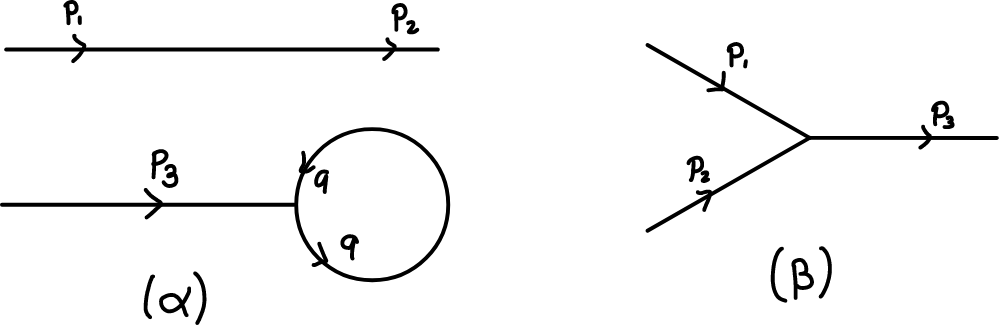
\includegraphics[width=0.5\textwidth]{figures/ex3-p3o1.png}
    \caption{The two diagrams for the first order contribution to the three-point correlation function. Diagram $(\alpha)$ shows the first option, where two external fields contract with each other, and the third contracts with one of the internal fields. We can see in the diagram that $p_3$ must vanish, and so we can ignore this diagram. Diagram $(\beta)$ shows the second option, where each external field contracts with a different internal field.}
\end{figure}
So, we are left only with only one vertex, no propegators, and three external lines matching $p_1, p_2, p_3$. There are no undetermined momenta:
\begin{equation}
    \bra{\Omega} T \tilde{\phi}(p_1)\tilde{\phi}(p_2)\tilde{\phi}(p_3) \ket{\Omega} = -i\mu \delta(p_1 + p_2 + p_3)
\end{equation}
\FloatBarrier
\subsection{Next order contribution}
The next order contribution will have to come from $\mu^3$, since for even orders there is an odd number of fields, resulting in one of the fields being left alone, not to be contracted with any other field.
\newline
This time, we need to contract three external fields with nine internal fields, along three vertices. First, we can look at the same diagrams as the first case, with the addition of vaccum loops. These loops are of order $\mu^2$ and thus have two vertices, and so include two diagrams: the glasses diagram and the fully connected diagram (every line is between the same two points). We can ignore those.This gives four diagrams:
\begin{itemize}
    \item The first is the unconnected diagram: each field contracts with one of the internal fields, creating three lolipop shapes. These require all momenta to be zero, and can therefore also be ignored.
    \item The second is the four-points second order correlation function where one of the points is an internal field contracted with itself. In this diagram, there is a central vertex leading to three distinct subdiagrams: one is just an external field, another is a vertex betwen the two remaining external fields, and the last is a loop with the last vertex.
    \item The third is just the first order connected diagram with a loop on one of the lines, adding two vertices.
    \item The last one is the three point loop diagram, where there is a circle and from three different points on the circle there are three different vertices connected each to an external field
\end{itemize}
\begin{figure}[!htbp]
    \centering
    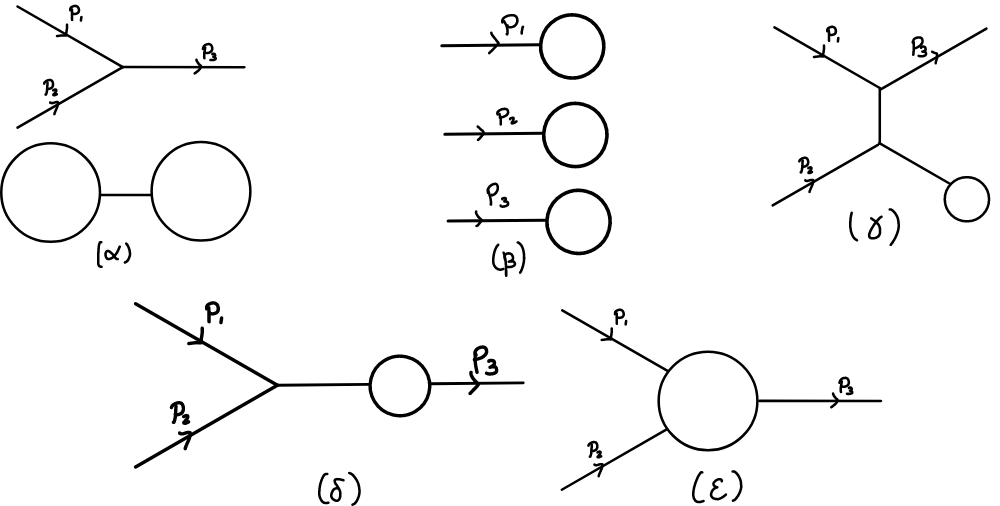
\includegraphics[width=0.7\textwidth]{figures/ex3-p3o3.png}
    \caption{Five diagrams for the third order contribution to the three-point correlation function. Diagram $(\alpha)$ is an example of a vaccum loop addition to the first order diagram, in this case the glasses diagram. $(\beta)$ is the three lolipop diagram, where each external field contracts with a different internal field. $(\gamma)$ is the second diagram, where one of the internal fields in the second order four-points correlation function is contracted with itself. $(\delta)$ is the third diagram, where we have a loop on one of the lines in the first order diagram. Finally, $(\varepsilon)$ xis the three point loop diagram.}
\end{figure}
\FloatBarrier
\subsection{Symmetry factors}
For each of the last three diagrams in the last section, we can find the symmetry factor:
\begin{itemize}
    \item For $(\gamma)$, has no symmetry, since each of the two "identical" vertices connects to external momenta, which are distinguishable. So the symmetry factor here is $S_\gamma = 1$
    \item For $(\delta)$, the two lines in the loop can be exchanged, giving a symmetry factor of $S_\delta = 2$.
    \item For this one, the internal three lines in the loop can be enumerated, giving a symmetry factor of $S_\varepsilon = 3! = 6$.
\end{itemize}
\subsection{Four points correlation function}
This time, since there is a even number of fields, the odd orders will vanish. So, we will calculate it up to second order. This leaves us with the zeroth order, which is just the free four-points correlation function:
\begin{equation}
\begin{gathered}
    \bra{\Omega} T \tilde{\phi}(p_1)\tilde{\phi}(p_2)\tilde{\phi}(p_3)\tilde{\phi}(p_4) \ket{\Omega}|_{\mu = 0} = \Delta_F(x_1 - x_2)\Delta_F(x_3 - x_4) + \\ + \Delta_F(x_1 - x_3)\Delta_F(x_2 - x_4) + \Delta_F(x_1 - x_4)\Delta_F(x_2 - x_3)
\end{gathered}
\end{equation}
And the second order, which includes two internal momenta
\begin{equation}
    \tilde{\phi}(p_1)\tilde{\phi}(p_2)\tilde{\phi}(p_3)\tilde{\phi}(p_4)
    \tilde{\phi}(q_1)\tilde{\phi}(q_1)\tilde{\phi}(q_1)
    \tilde{\phi}(q_2)\tilde{\phi}(q_2)\tilde{\phi}(q_2)
\end{equation}
the following diagrams:
\begin{itemize}
    \item The first case where the vertices are connected amongst themselves, and the external fields are contracted with eachother. This is just a vaccum loop extension of the zeroth order, so we can ignore it.
    \item Three out of four fields contract with the same vertex, and the last field is on the other vertex.
    \begin{equation}
        \contraction[0.25em]{}{\tilde{\phi}}{(p_1)\tilde{\phi}(p_2)\tilde{\phi}(p_3)\tilde{\phi}(p_4)}{\tilde{\phi}}
        \contraction[0.5em]{\tilde{\phi}(p_1)}{\tilde{\phi}}{(p_2)\tilde{\phi}(p_3)\tilde{\phi}(p_4)\tilde{\phi}(q_1)}{\tilde{\phi}}
        \contraction[0.75em]{\tilde{\phi}(p_1)\tilde{\phi}(p_2)}{\tilde{\phi}}{(p_3)\tilde{\phi}(p_4)\tilde{\phi}(q_1)\tilde{\phi}(q_1)}{\tilde{\phi}}
        \contraction[1em]{\tilde{\phi}(p_1)\tilde{\phi}(p_2)\tilde{\phi}(p_4)}{\tilde{\phi}}{(p_4)\tilde{\phi}(q_1)\tilde{\phi}(q_1)\tilde{\phi}(q_1)}{\tilde{\phi}}
        \contraction[0.5em]{\tilde{\phi}(p_1)\tilde{\phi}(p_2)\tilde{\phi}(p_3)\tilde{\phi}(p_4)\tilde{\phi}(q_1)\tilde{\phi}(q_1)\tilde{\phi}(q_1)\tilde{\phi}(q_2)}{\tilde{\phi}}{(q_2)}{\tilde{\phi}}
        \tilde{\phi}(p_1)\tilde{\phi}(p_2)\tilde{\phi}(p_3)\tilde{\phi}(p_4)
        \tilde{\phi}(q_1)\tilde{\phi}(q_1)\tilde{\phi}(q_1)
        \tilde{\phi}(q_2)\tilde{\phi}(q_2)\tilde{\phi}(q_2)
    \end{equation}
    In this contraction we again get that one of the momenta is zero, and so we ignore it.
    \item Finally, we have contractions where each two fields contract with one internal field, and the two internal fields contract with the other. There are three options of how to group the external momenta into the two vertices, resulting in three Feynman diagrams.
    \begin{equation}
        \contraction[0.25em]{}{\tilde{\phi}}{(p_1)\tilde{\phi}(p_2)\tilde{\phi}(p_3)\tilde{\phi}(p_4)}{\tilde{\phi}}
        \contraction[0.5em]{\tilde{\phi}(p_1)}{\tilde{\phi}}{(p_2)\tilde{\phi}(p_3)\tilde{\phi}(p_4)\tilde{\phi}(q_1)}{\tilde{\phi}}
        \contraction[0.75em]{\tilde{\phi}(p_1)\tilde{\phi}(p_2)}{\tilde{\phi}}{(p_3)\tilde{\phi}(p_4)\tilde{\phi}(q_1)\tilde{\phi}(q_1)\tilde{\phi}(q_1)}{\tilde{\phi}}
        \contraction[1em]{\tilde{\phi}(p_1)\tilde{\phi}(p_2)\tilde{\phi}(p_4)}{\tilde{\phi}}{(p_4)\tilde{\phi}(q_1)\tilde{\phi}(q_1)\tilde{\phi}(q_1)\tilde{\phi}(q_2)}{\tilde{\phi}}
        \contraction[0.5em]{\tilde{\phi}(p_1)\tilde{\phi}(p_2)\tilde{\phi}(p_3)\tilde{\phi}(p_4)\tilde{\phi}(q_1)\tilde{\phi}(q_1)}{\tilde{\phi}}{(q_1)\tilde{\phi}(q_2)\tilde{\phi}(q_2)}{\tilde{\phi}}
        \tilde{\phi}(p_1)\tilde{\phi}(p_2)\tilde{\phi}(p_3)\tilde{\phi}(p_4)
        \tilde{\phi}(q_1)\tilde{\phi}(q_1)\tilde{\phi}(q_1)
        \tilde{\phi}(q_2)\tilde{\phi}(q_2)\tilde{\phi}(q_2)
    \end{equation}
\end{itemize}
\FloatBarrier
\begin{figure}[!htbp]
    \centering
    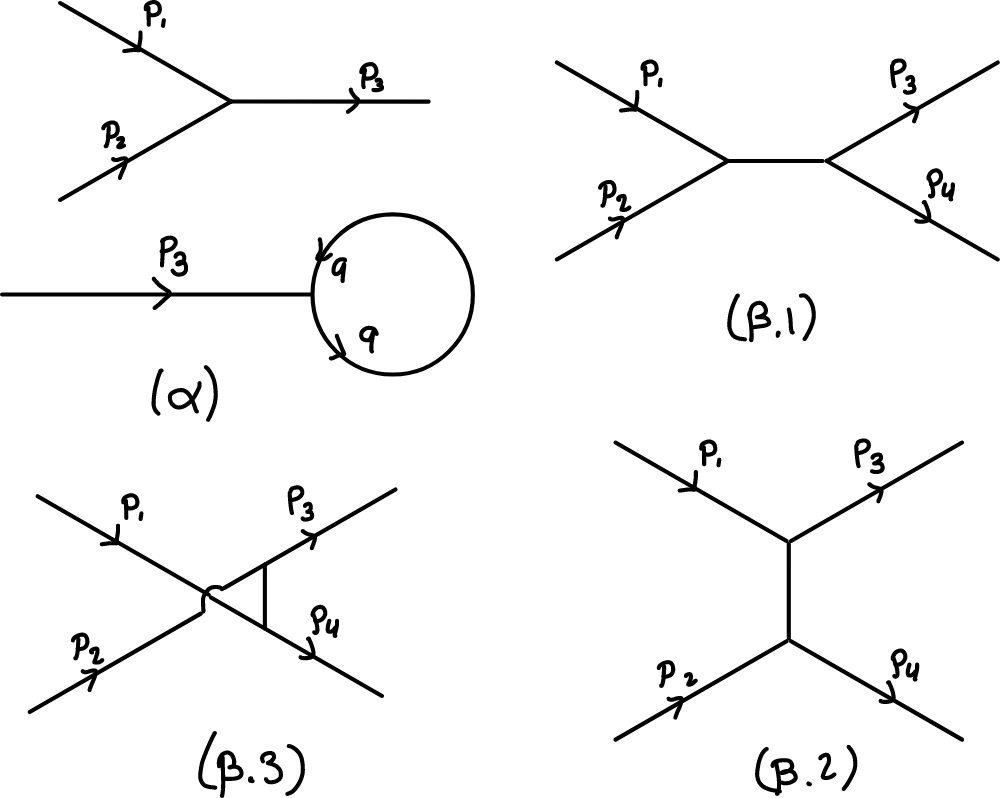
\includegraphics[width=0.7\textwidth]{figures/ex3-p4o2.png}
    \caption{The four second order diagrams that are not vaccum loop extension of the first order. Diagram $(\alpha)$ shows the option where three fields contract with the same vertex, and the last field is on the other vertex, causing it to be zero. This is very similar to the case we had in the three-point correlation function in first order. The other three diagrams $(\beta.1)$, $(\beta.2)$ and $(\beta.3)$ show the other three options of how to contract the four fields with two internal fields.}
\end{figure}
\FloatBarrier
So, there are three connected diagrams, one for each possible pairing of momenta. In each of them, we get two delta functions including an internal momenta $q$ for the propegator between the two vertices. We can use one of the delta functions to solve the integral and get:
\begin{equation}
\begin{gathered}
    \bra{\Omega} T \tilde{\phi}(p_1)\tilde{\phi}(p_2)\tilde{\phi}(p_3)\tilde{\phi}(p_4) \ket{\Omega} = \bra{\Omega} T \tilde{\phi}(p_1)\tilde{\phi}(p_2)\tilde{\phi}(p_3)\tilde{\phi}(p_4) \ket{\Omega}|_{\mu=0} - \\
    -i\mu^2 \Bigg[\frac{\delta(p_1 + p_2 - p_3 - p_4)}{\left(p_1 + p_2\right)^2 - m^2 + i\epsilon} + \frac{\delta(p_1 + p_3 - p_2 - p_4)}{\left(p_1 + p_3\right)^2 - m^2 + i\epsilon} + \frac{\delta(p_1 + p_4 - p_2 - p_3)}{\left(p_1 + p_4\right)^2 - m^2 + i\epsilon}
    \Bigg]
\end{gathered}
\end{equation}
\subsection{Next order contribution}
Again, the next order will be two orders above, meaning the $\mu^4$ order. This includes all diagrams with four vertices.
\begin{itemize}
    \item First, we can add a loop to the connected diagram of the second order four-points correlation function. We can add this loop either in the internal propegator or on one of the external lines. This gives us two topoloigcally distinct diagrams.
    \item Next, we have the four points loop diagram, which is just a circle with four vertices in four points, each connected to a different external momenta.
    \item Finally, there is the taking the three point loop diagram, and splitting one of its legs into two external momenta, adding a vertex and a momenta.
\end{itemize}
\FloatBarrier
\begin{figure}[!htbp]
    \centering
    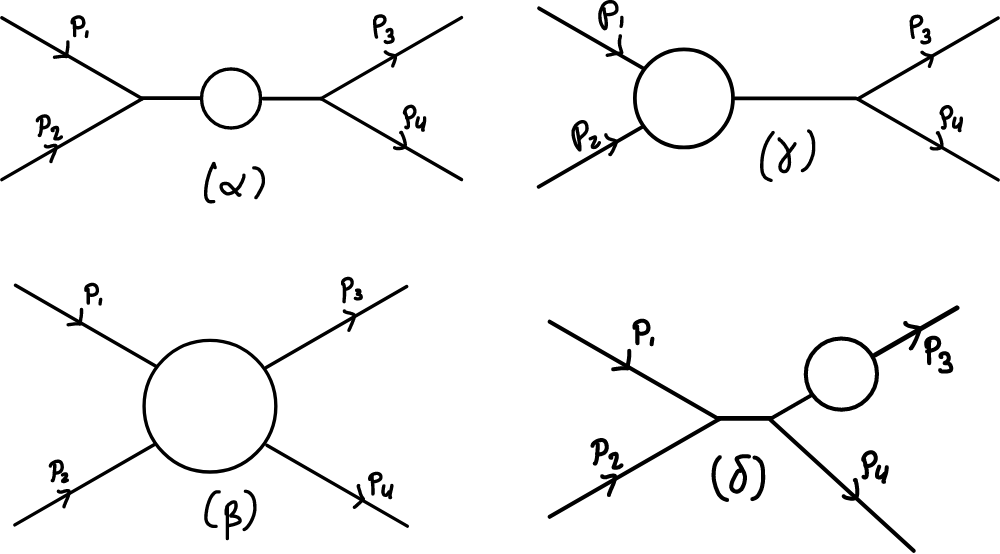
\includegraphics[width=0.7\textwidth]{figures/ex3-p4o4.png}
    \caption{The fourth order diagrams contrbuting to the four point correlation function. Diagrams $(\alpha)$ and $(\delta)$ show the two options of adding a loop to the second order connected diagram. Diagram $(\gamma)$ shows the four points loop diagram, and diagram $(\beta)$ shows the option of taking the three point loop diagram and splitting one of its legs into two external momenta.}
\end{figure}
\FloatBarrier
\subsection{The "glasses" diagram symmetry factor}
The glasses diagram has a symmetry factor of 8: factor two from the flipping of each loop, and another factor 2 from the interchangability of the internal vertices.
\end{document}